\documentclass[simplex.tex]{subfiles}
% NO NEED TO INPUT PREAMBLES HERE
% packages are inherited from simplex.tex; you can compile this on its own

\onlyinsubfile{
\title{NeuroData SIMPLEX Report: Subfile}
}

\begin{document}
\onlyinsubfile{
\maketitle
\thispagestyle{empty}

The following report documents the progress made by the labs of Randal~Burns and Joshua~T.~Vogelstein at Johns Hopkins University towards goals set by the DARPA SIMPLEX grant.

%%%% Table of Contents
\tableofcontents

%%%% Publications
\bibliographystyle{IEEEtran}
\begin{spacing}{0.5}
\section*{Publications, Presentations, and Talks}
\vspace{-20pt}
\nocite{*}
{\footnotesize	\bibliography{simplex}}
\end{spacing}
%%%% End Publications
}


\subsection{ndviz}

Several small ndviz interface adjustments were introduced. First and foremost, a scale bar was added to the viewer screen. Additional visual tweaks and bug fixes were made, and a new beta release was published\footnote{\href{http://viz.neurodata.io}{http://viz.neurodata.io}}.

The ndviz backend system was re-engineered to incorporate the React javascript library. React speeds up dynamic javascript client code by only making necessary adjustments to the Document Object Model (DOM). Updating the DOM is a slow process. To speed updating, React builds a virtual DOM. With each change, React checkpoints the virtual DOM, builds a new virtual DOM, and compares the two. Based on the comparison, changes are applied to the real DOM. Although this process is more complex, building the virtual DOM is much faster than making wide-ranging updates to the real DOM. 


React also decouples the ndivz viewer state from form fields and user controls. For example, the state of the opacity sliders is now set by backend javascript code, and the sliders are updated on each open, or on user interaction. By handling application in backend code, the user facing state is always consistent. And, the groundwork is now in place to save the complete application state for each user session, allowing a user to set a number of image processing parameters and resuming their session with all parameters restored at a later time. 


Finally, both the bounding box and the query by key ndramondb queries
were added to ndviz. Ndviz can now center on an arbitrary annotation, as
well as list all annotations by type for a given project (see Figure
\ref{fig:ndviz}).
\begin{figure}[h!]
\begin{cframed}
\centering
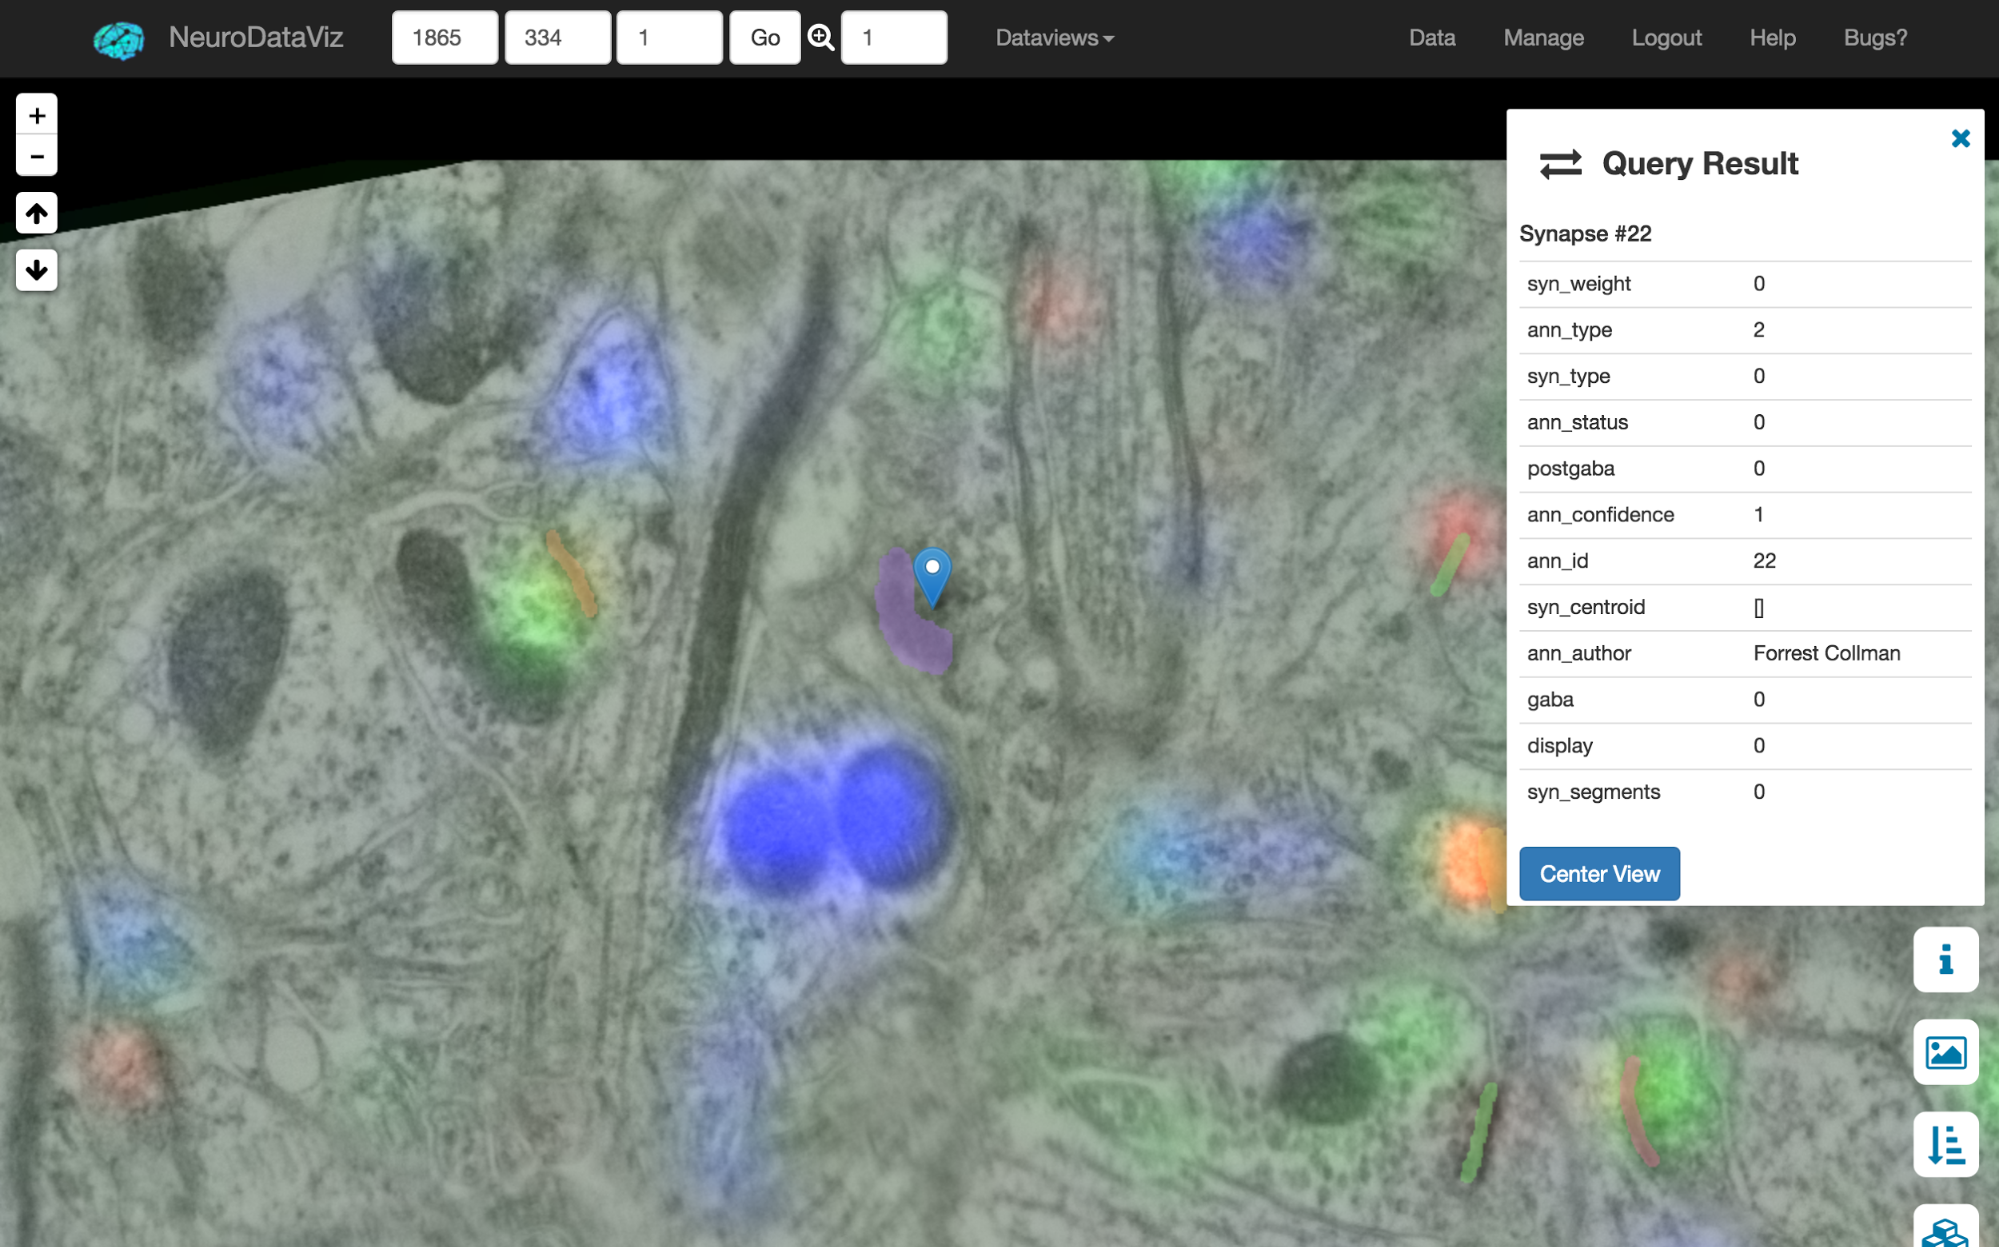
\includegraphics[width=\textwidth]{./figs/ndviz.png}
\caption{ndviz displaying an annotation project (Array Tomography with conjugate Electron Microscopy) with Synapse \#22 centered (blue marker). 
The figure was obtained by loading 
\href{http://synaptomes.neurodata.io/ndv/project/collman15_annotations/xy/1/1590/1069/0/}{annotations}, selecting Synapse \#22 in the Query Tool box (magnifying glass, picture below), and clicking the blue ``Center View'' button. 
}
\label{fig:ndviz}
\end{cframed}
\end{figure}


\begin{figure}[h!]
\begin{cframed}
\centering
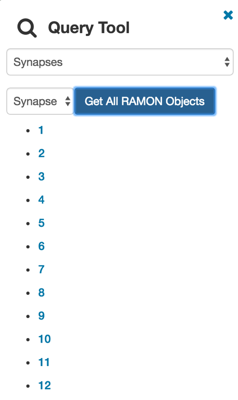
\includegraphics[width=.25\textwidth]{./figs/ndviz-query.png}
\caption{The \itshape{ndviz} Query Tool controls box. Clicking a blue Synapse ID
  will open the Query Result box in the viewer, and allow the user to
  center the current view on the selected annotation.}
\label{fig:ndviz-query}
\end{cframed}
\end{figure}

\end{document}
